

\chapter{Overview NLO}




\textbf{SHG, phase matching
}
SHG efficiency as function of angle / temperature
determine crystal orientation / model data from crystal orientation

\textbf{FWM}
Model data

\textbf{Pulse shaper:} linear + nonlinear, CEP and without

Pump-probe, 2D ?

THG

Frog etc.



Wir untersuchen systhematisch die kohärente Wechselwirkung
von mehreren Lichtpulsen mit einer Probe. Mir gefällt hier
das Skript von P.~Hamm am besten.

\section{10.1. Wdh. Liouville-Gleichung\protect\footnote{Hamm 2005, Kap. 1}\hfill w} 

Das ist  die Schrödinger-Gleichung für Dichte-Matrix, inkl.
Zerfallsprozessen. Eigentlich nur eine elegante
Schreibweise.

Unter Verwendung gewöhnlicher Zustände findet man

\begin{equation}
    \frac{\partial}{\partial t}|\psi\rangle = -\frac{i}{\hbar}|\psi\rangle
\end{equation}

Beschreibt man das System nicht mit $|\psi\rangle$, sondern mit der Dichtematrix $\rho = |\psi\rangle\langle\psi|$, so findet man für deren Zeitentwicklung die Louville-Gleichung

\begin{equation}
     \frac{\partial}{\partial t}\rho = -\frac{i}{\hbar}[H,\rho]
\end{equation}

Wählt man eine Basis von Zuständen $|1\rangle$ und $|2\rangle$, so können die Elemente von $\rho$ beschrieben werden durch

\begin{equation}
    \rho_{nm} = c_nc_m*
\end{equation}

Wenn $|\psi\rangle = c_1|1\rangle + c_2|2\rangle$

Der Vorteil der Dichtematrix-Notation liegt darin, dass jetzt nicht nur kohärente Überlagerungen von Basiszuständen $\frac{1}{\sqrt{2}}(|1\rangle + |2\rangle)$ beschreiben werden können, sondern auch statistische Gemische von Zuständen 

\begin{equation}
    \rho = \sum_k|\psi_k\rangle\langle\psi_k|
\end{equation}

Dies ist insbesondere Desewegen möglich, da die Louville Gleichung linear ist. 

\section{10.2. Perturbative Expansion\protect\footnote{Hamm 2005, Kap. 2}\hfill *}

Das Auf-Integrieren der Schrödinger-Gleichung ist schwierig.
Es wird einfacher, wenn man von kleinen, zeitlich separaten
Störungen (= Laser-Pulsen) ausgeht. 

Zur Beschreibung der Zeitentwicklung von $\psi$ können sogenannte Zeitentwicklungsoperatoren $U$ verwendet werden mit

\begin{equation}
    \psi(t) = U(t,t_0)\psi(t_0)
\end{equation}

Es kann gezeigt werden, dass gilt

\begin{equation}
    \frac{\partial}{\partial t}U(t,t_0) = -\frac{i}{\hbar}H\cdot U(t,t_0)
\end{equation}

bzw.

\begin{equation}
    U(t,t_0) = e^{-\frac{i}{\hbar}H(t-t_0)}
\end{equation}

Ziel ist es hier die Wechselwirkung mit einem Externen Lichtfeld zu beschreiben. Beschrieben wird das Problem im Folgenden über das sogenannte Wechselwirkungsbild. Hier wird ein Hamilton-Operator mit kleiner Störung wie folgt angenommen

\begin{equation}
    H = H_0 + H'(t)
\end{equation}

Hier wird angenommen, dass $H_0$ zeitunabhängig und $H'(t)$ zeitabhängig ist (Wechselwirkungsbild). Der zu $H_0$ gehörende Zeitentwicklungsoperator ist $U_0$. Nun tragen zwei Effekte zur Zeitentwicklung von $\psi(t)$ bei. Zum einen entwickelt sich $\psi$ durch die Wirkung von $H_0$ und zum Anderen durch den Einfluss von $H'(t)$. Formal wird dies durch die Wellenfunktion im WW-Bild $\psi_I$ dargestellt. 

\begin{equation}
    \psi(t) = U_0(t,t_0)\psi_I(t)
\end{equation}

Die Zeitentwicklung durch $H_0$ wird über $U_0$ vermittelt und die Entwicklung von $\psi_I(t)$ geht nur auf $H'(t)$ zurück.

Mit Def.:

\begin{equation}
    H_I'(t) = U_0^{\dagger}(t,t_0)H'(t)U_0(t,t_0)
\end{equation}

kann gezeigt werden, dass gilt

\begin{equation}
    \frac{\partial}{\partial t}\psi_I(t) = -\frac{i}{\hbar}H_I'(t)\cdot\psi_I(t)
\end{equation}

Analog kann für die Dichtematrix gezeigt werden, dass gilt

\begin{equation}
    \frac{\partial}{\partial t}\rho_I(t) = -\frac{i}{\hbar}[H_I'(t)\cdot\rho_I(t)]
\end{equation}

Wobei hier $\rho_I$ aus den Wellenfunktionen im WW-Bild gebildet wird. Integration von Gl. (87) liefert

\begin{equation}
    \psi_I(t) = \psi_I(t_0) = \sum_{n=1}^{\infty}(-\frac{i}{\hbar})^n\int_{t_0}^{t}d\tau_n\int_{t_0}^{\tau_n}d\tau_{n-1}(...)\int_{t_0}^{\tau_2}d\tau_1H'_I(\tau_n)(...)H'_I(\tau_1)\psi_I(t_0)
\end{equation}

Verwendet man die (Gl. 85), und die Wellenfunktion Nullter Ordnung,

\begin{equation}
    \psi^{(0)}(t) = U(t,t_0)\psi(t_0)
\end{equation}

so findet man:

\begin{equation}
    \psi(t) = \psi^{(0)}(t) + \sum_{n=1}^{\infty}(-\frac{i}{\hbar})^n\int_{t_0}^{t}d\tau_n\int_{t_0}^{\tau_n}d\tau_{n-1}(...)\int_{t_0}^{\tau_2}d\tau_1U_0(t,\tau_n)H'_I(\tau_n)(...)U_0(\tau_2,\tau_1)H'_I(\tau_1)U_0(\tau_1,t_0)\psi_I(t_0)
\end{equation}

Analoge Überlegungen sind auch für die Dichtematrix möglich.



\section{10.3. Nichtlineare  Suszeptibilität\protect\footnote{Hamm 2005, Kap. 2}\hfill *} 

Ein klein wenig nichtlineare Optik. Wie würde man ohne QM
die Wechselwirkung von mehreren Feldern mit Materie
beschreiben?

Die dielektrische Verschiebung ist definiert gemäß:

\begin{equation}
    \vec{D} = \epsilon_0\vec{E} + \vec{P}
\end{equation}

In erster Näherung steht die Polarisation $\vec{P}$ in linearer Beziehung mit dem elektrischen Feld:

\begin{equation}
    P = \epsilon_0\chi^{(1)}E
\end{equation}

Tatsächlich ist der Zusammenhang jedoch nichtlinear mit:

\begin{equation}
    P = \epsilon_0(\chi^{(1)}\cdot E + \chi^{(2)}\cdot E\cdot E + \chi^{(3)}\cdot E\cdot E\cdot E + ...)
\end{equation}

Andererseits ist die makroskopische Polarisation gegeben durch:

\begin{equation}
    \langle P(t)\rangle = \langle \mu\rho(t)\rangle = \rho_{12}\mu_{21} + \rho_{21}\mu_{12}
\end{equation}

Mit $\rho(t) = \rho^{(0)} + \sum_{n=1}^{\infty}\rho^{(n)}(t)$ und (Gl. 94) findet man:

\begin{equation}
    P^{(n)}(t) = \langle \mu\rho^{(n)}(t)\rangle
\end{equation}

\section{10.4. Double-sided Feynman diagrams\protect\footnote{Hamm 2005, Kap. 3}\hfill ***} 

\textit{Ein sehr mächtiges Werkzeug, um  alle Permutationen von
Wechselwirkungs-Reihenfolgen zu erfassen und deren Folge zu
berechnen.}\\
\textbf{Regeln:}
\begin{itemize}
    \item vertikale Linien repräsentieren die Zeitentwicklung von ket (links) und bra (rechts) der Dichte-Matrix. Die Zeit läuft von unten nach oben.
    \item Die Wechselwirkungen mit einem Lichtfeld werden mit Pfeilen gekennzeichnet. Die letzte Wechselwirkung unterscheidet sich vom Rest und wird daher gesondert gekennzeichnet.
    \item Jeden Diagramm besitzt ein Vorzeichen $(-1)^n$, wobei $n$ die Anzahl der Wechselwirkungen von der rechten Seite ist, da diese jeweils ein Minus im Kommutator bedeuten. \footnote{Wie kann eine Wechselwirkung Teil oder Nicht-Teil des Kommutators sein?}
    \item Ein Pfeil nach rechts repräsentiert ein elektrisches Feld $e^{-i \omega t + ikr}$, während ein Pfeil nach links für ein el. Feld $e^{+i \omega t - ikr}$ steht. Das emittierte Licht, z.B. die letzte Wechselwirkung, hat die Frequenz und den Wellenvektor, welche die Summen der Input-Frequenzen und -Wellenvektoren sind.
    \item Ein Pfeil, der zum System hin zeigt, repräsentiert ein Ansteigen der entsprechenden Seite der Dichte-Matrix, ein Pfeil weg vom System dagegen eine De-Excitation. Diese Regel ist eine Folge der rotating wave approximation. Da die letzte Wechselwirkung im Normalfall eine Emission ist, zeigt sie immer weg vom System.
    \item Die letzte Wechselwirkung muss in einem bevölkerten Zustand \footnote{population state?} enden.
\end{itemize}
\paragraph{Beispiel 1:} Nichtlineare Antwort dritter Ordnung
\begin{figure} [h]
    \centering
    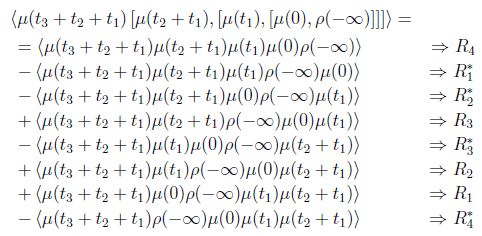
\includegraphics[width = 0.7 \textwidth]{\currfiledir/Feynman1.JPG}
    \caption{Terme der Nichtlinearen Antwort dritter Ordnung}
    \label{fig:Feynman1}
\end{figure}
\begin{figure} [h]
    \centering
    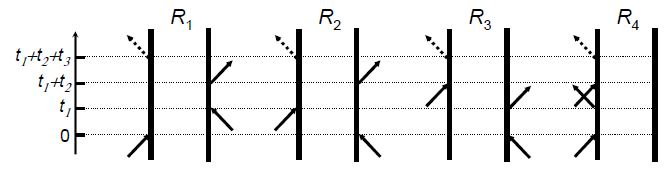
\includegraphics[width = 0.9 \textwidth]{\currfiledir/Feynman2.JPG}
    \caption{resultierendes Feynman-Diagramm}
    \label{fig:Feynman2}
\end{figure}

\paragraph{Beispiel 2:} drei zeitlich versetzte Laserpulse (siehe Abb. \ref{fig:Feynman3})

\begin{figure} [h!]
    \centering
    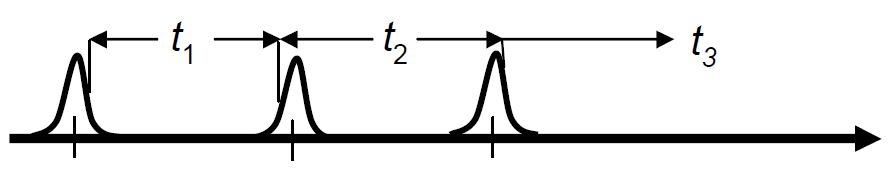
\includegraphics[width = 0.9 \textwidth]{\currfiledir/Feynman3.JPG}
    \caption{Pulsabfolge}
    \label{fig:Feynman3}
\end{figure}

Das sich ergebende E-Feld ist die Summe aus den drei einzelnen Pulsen.
\begin{equation}
    E(t) = E_1(t)\cdot(e^{-i\omega t} + e^{+i\omega t}) + E_2(t)\cdot(e^{-i\omega t} + e^{+i\omega t}) + E_3(t)\cdot(e^{-i\omega t} + e^{+i\omega t})
\end{equation}
Daraus würde folgen, dass insgesamt 6$\cdot$6$\cdot$6$\cdot$4=864 Terme berücksichtigt werden müssten.\\
Diese Zahl kann durch Tricks vermindert werden:
\begin{enumerate}
    \item \textbf{Time ordering:} Die Reihenfolge der Pulse wird berücksichtigt. Das schränkt die Anzahl der Terme auf 32 ein.
    \item \textbf{Rotating Wave Approximation:} Entweder $e^{-i\omega t}$- oder $e^{+i\omega t}$-Terme tragen bei, aber nie beide gleichzeitig. Die Anzahl der Terme beträgt noch 4.
    \item \textbf{Phase Matching:} Jetzt werden zusätzlich noch die Wellenvektoren mitgenommen. Das E-Feld wird zu
    \begin{align}
    E(t) &= E_1(t)\cdot(e^{-i\omega t+ikr} + e^{+i\omega t-ikr}) + E_2(t)\cdot(e^{-i\omega t+ikr} + e^{+i\omega t-ikr}) \notag\\ &+ E_3(t)\cdot(e^{-i\omega t+ikr} + e^{+i\omega t-ikr})
     \end{align}
     Daraus folgt, dass es zwei verschiedene Möglichkeiten zur Aufsummierung der k-Vektoren gibt $k = k_1 \pm k_2 \pm k_3$, wobei nur eine Option am Ende überlebt.
     \begin{figure} [h]
    \centering
    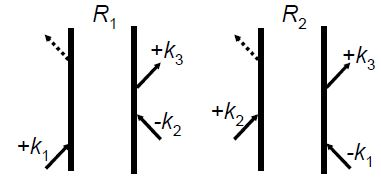
\includegraphics[width = 0.9 \textwidth]{\currfiledir/Feynman4.JPG}
    \caption{Die beiden Möglichkeiten, die Wellenvektoren aufzusummieren.}
    \label{fig:Feynman4}
\end{figure}
\end{enumerate}
Am Ende sind nur noch \textbf{zwei} Komponenten zu beachten.


\section{10.5. Pump-Probe Spectroscopy\protect\footnote{Hamm 2005,  Kap. 4.1}\hfill **} 

Wie beschreibt man mit dem eben eingeführten Formalismus
Zwei-Puls-Experimente?


\section{10.6. {2D}-Spektroskopie\protect\footnote{Hamm 2005, Kap. 7}\hfill ***} 

Wie beschreibt man 3-Puls-Experimente? Wie findet man so
Kopplung zwischen Zuständen, nicht nur Eigenenergien?
 
